\documentclass{article}
\usepackage{graphicx} 
\usepackage{amsmath, amsthm, amssymb, amsfonts}
\usepackage{float}
\usepackage{titlesec}
\usepackage{geometry}
\usepackage{pgfplots}
\usepackage{ragged2e}
\usepackage{circuitikz}
\usepackage{ragged2e}
\usepackage{showlabels}
\usepackage{siunitx}
\usepackage{booktabs}
\usepackage[italian]{babel}
\newcommand{\showlabel}[1]{\textbf{#1}\label{#1}}
\geometry{
    a4paper,
    total={170mm,257mm},
    left=20mm,
    top=20mm,
}

\begin{document}
\justifying

\begin{center}
    {\fontsize{36}{43.2}\selectfont Relazione di laboratorio 3 - Gruppo D6/D10}
\end{center}
\noindent
\textbf{Componenti gruppo:} Cortese Riccardo, Lana Mirko

\section*{Materiale Utilizzato e circuito usato per l'esperienza}

Durante l'esecuzione del laboratorio è stato utilizzato il seguente materiale:
\begin{itemize}
    \item breadboard;
    \item cavi bnc, banana-banana e banana-bnc;
    \item resistori \((1k\Omega, 10k\Omega)\);
    \item capacitori \((1nF, 10nF, 100nF)\);
    \item decade di induttanze;
    \item filetti;
    \item generatore di forme d'onda;
    \item oscilloscopio.
\end{itemize}

\begin{figure}[h!]
\centering
\resizebox{0.35\textwidth}{!}{
    \begin{circuitikz}
        % Vin source
        \draw (0,0) to[vsourcesin, l=$V_{\text{in}}(t)$] (0,3) 
            -- (2,3) 
            to[C, l=$C$] (4,3) 
            to[L, l=$L$] (6,3)
            -- (8,3) 
            to[R, l=$R$] (8,0) 
            -- (0,0);
    
        % Ground connection
        \draw (8,0) node[ground] {};
    
        % Vout connection
        \draw (8,3) -- ++(1,0) node[above] {$+$};
        \draw (8,0) -- ++(1,0) node[below] {$-$};
        \node[right] at (9,1.5) {$V_{\text{out}}(t)$};
    \end{circuitikz}
    }
    \caption{Circuito per l'Esercizio 1 e 2}
    
\end{figure}

\section{Diagramma ingresso-uscita (Diagramma di Bode)}

\subsection{Obiettivo}
Con riferimento al circuito di \textit{Figura 1} utilizzando le seguenti combinazioni di R, L, C:
\begin{itemize}
    \item $R = 10 k\Omega, L = 500 mH$ e $C = 10 nF$;
    \item $R = 1 k\Omega, L = 500 mH$ e $C = 10 nF$;
\end{itemize}

si determini il diagramma di Bode del circuito. Si utilizzi una forma d'onda sinusoidale di ampiezza picco-picco $V_{in}^{pp} = 5 V$ con offset pari a zero ($V_{in}^{of} = 0 V$ ). Si utilizzino frequenze da 1 Hz a 50 kHz opportunamente scelte. Si misuri l'ampiezza della forma d'onda in entrata ($V_{in}^{p}$) ed uscita ($V_{out}^{p}$) e la differenza in fase tra le due forme d'onda. 

Si riportino i risultati in due grafici distinti.

Si verifichi se il comportamento del circuito è coerente con le aspettative.

Si stimi la resistenza parassita in serie all'induttore nel caso $R = 1 k\Omega, L = 500 mH$ e $C = 10 nF$.

\subsection{Dati sperimentali}
Di seguito riportiamo due tabelle contenenti le tensioni misurate ad ogni istante di tempo per le diverse combinazioni di R, L e C.

\begin{table}[H]
    \centering
    \begin{minipage}[t]{0.45\textwidth}
        \begin{center}
            \begin{tabular}{|c|c|c|}
                \hline
                Frequenza ($Hz$) & Vout (mV) & Ritardo ($\mu$s)\\
                \hline
                1 & 3.450 & \\
                2 & 6.126 & \\
                5 & 15.250 & \\
                10 & 30.250&\\
                20 & 61 & \\
                50 & 155 & \\
                100 & 301.250 &  \\
                200 & 607.500 &  \\
                500 & 1518 &  \\
                1000 & 2937 & \\
                2000 & 4650 & \\
                2250 & 4775 & \\
                4500 & 3387 & \\
                5000 & 3087 & \\
                10000 & 1506 & \\
                \hline
            \end{tabular}
            \caption{Dati prima combinazione RLC.}
        \end{center}
    \end{minipage}
    \hfill
    \begin{minipage}[t]{0.45\textwidth}
        \begin{center}
           \begin{tabular}{|c|c|c|}
                \hline
                Frequenza ($Hz$) & Vout (mV) & Ritardo ($\mu$s)\\
                \hline
                1 & 0 &\\
                2 & 0 &\\
                5 & 0.675 & \\
                10 & 1.300 & \\
                20 & 2.950 & \\
                50 & 7.875  & \\
                100 & 48.750 & 8079\\
                200 & 61.250 & 6167\\
                500 & 165.375 & 490\\
                1000 & 382.200 & 233\\
                2000 & 2199 & 67\\
                2020 & 2288 & \\
                2250 & 3236 & 1.950\\
                5000 & 397.700 & -254.47\\
                10000 & 159.500 & \\
                \hline
            \end{tabular}
            \caption{Dati seconda combinazione RLC.}
        \end{center}
    \end{minipage}
\end{table}

E' stato scelto di misurare la tensione \textit{$V_{out}$} ad intervalli di frequenza, nel range 1 Hz a 50 Hz, secondo una distribuzione logaritmica.

Oltre a questi dati è stata misurata la tensione \textit{$V_{out}$} nei punti di $f_0$ e $f_{-3db}$ per le due combinazione di R, L e C. 

I dati raccolti si fermano al raggiungimento di frequenza $f = 10 kHz$ in quanto, avendo a disposizione dei cavi lunghi come collegamento tra la decade di induttanze e la breadbord, essi introducevano una induttanza parassita che rendeva l'uscita (Vout) instabile e quindi difficile da misurare.

A puro scopo didattico, abbiamo provato a visualizzare il segnale d'uscita nell'oscilloscopio quando la frequenza $f = 50 kHz$ e abbiamo notato che ad ogni spostamento dei due fili che collegavano la decade di induttanze con la breadbord, il segnale in uscita mutava di volta in volta.

\subsection{Diagrammi di Bode}
Di seguito riportiamo i diagrammi di Bode, ampiezza e fase, relativi alle due combinazioni di R, L e C.

\noindent
I diagrammi sperimentali per l’ampiezza e per la fase si ottengono rispettivamente con le seguenti funzioni:

\begin{minipage} [t]{0.45\textwidth}
    \begin{equation}
        dB = 20log \bigg ( \frac{V_{out}}{V_{in}} \bigg)
    \end{equation}
\end{minipage}
\hfill
 \begin{minipage} [t]{0.45\textwidth}
    \begin{equation}
        \phi[rad] = \frac{\Delta t}{2 \pi \cdot T} 
    \end{equation}
\end{minipage}

 
\begin{figure}[H]
    \centering
    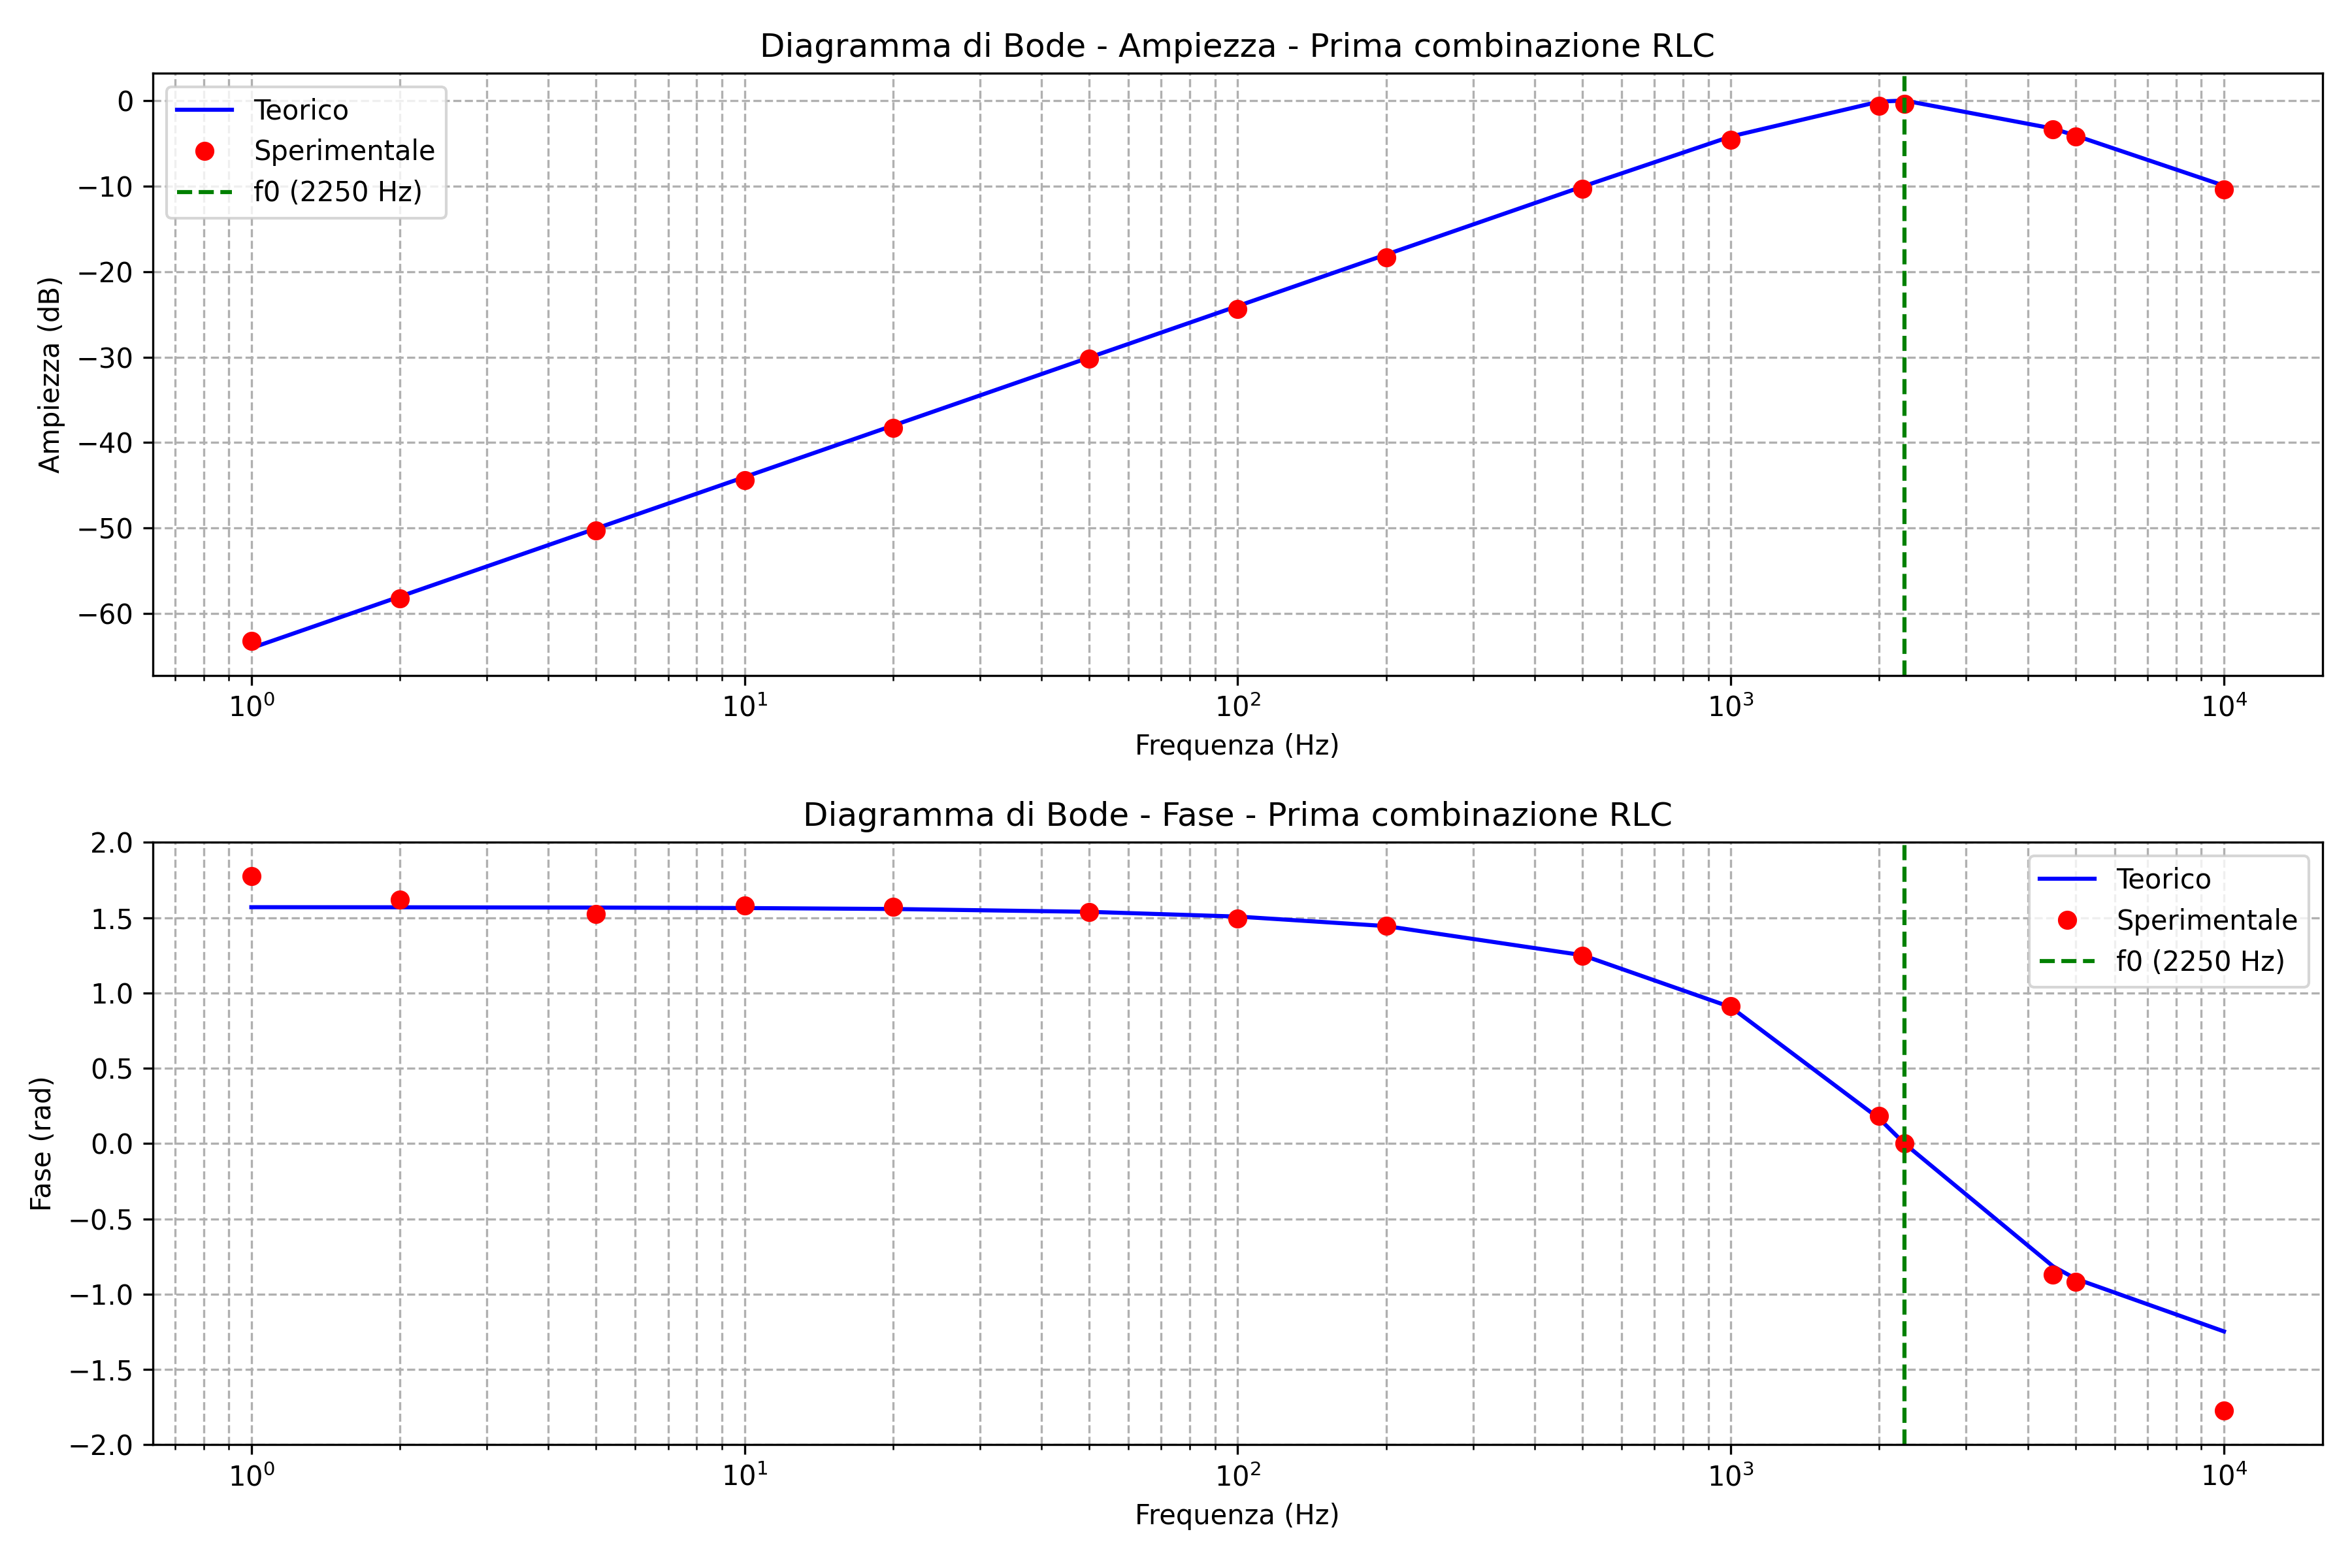
\includegraphics[width=0.8\linewidth]{figures/diagramma_bode_1.png}
\end{figure}
\noindent

\begin{figure}[H]
    \centering
    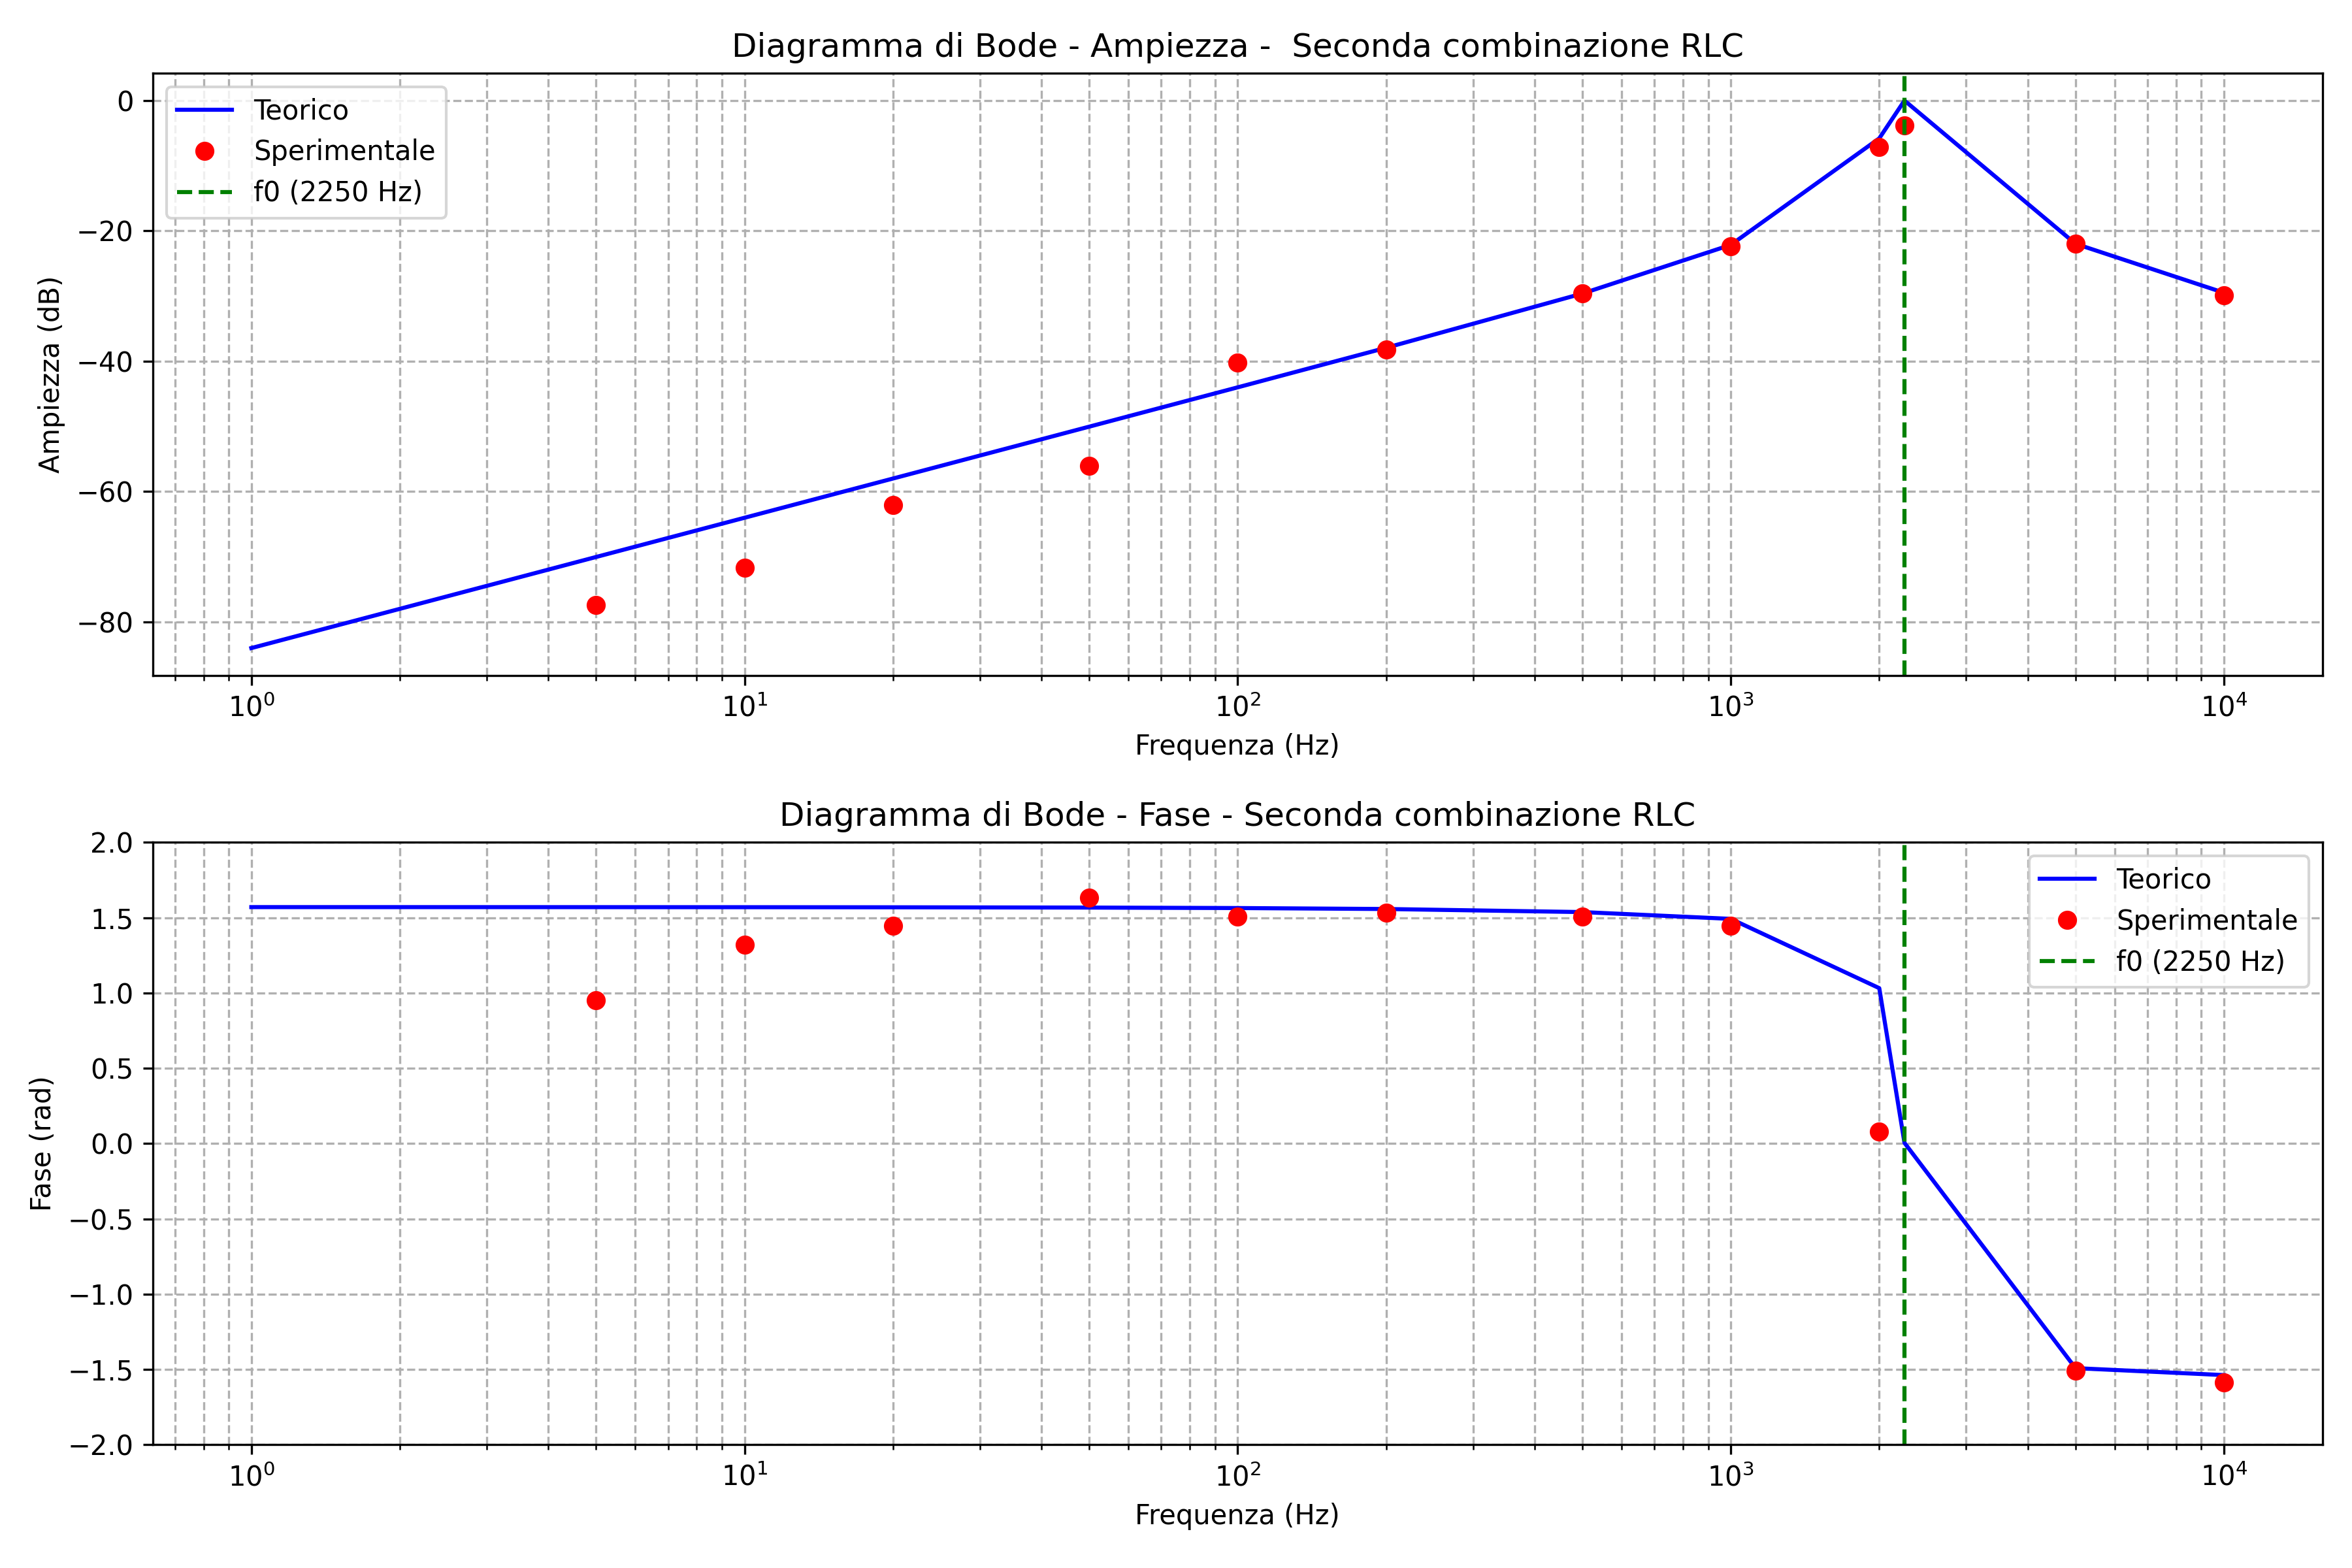
\includegraphics[width=0.8\linewidth]{figures/diagramma_bode_2.png}
\end{figure}
\noindent

I diagrammi sono stati generati tramite codice python da noi implementato.

\subsection{Conclusioni}
Dopo aver calcolato e riportato i diagrammi di Bode per le rispettive combinazioni R, L, e C, possiamo notare come nel primo caso i dati sperimentali rispecchiano l'andamento della curava teorica, a meno di errori sperimentali; nel secondo caso i punti relativi ai dati sperimentali appaiono sottostanti la curva teorica e inoltre a $f_0$ la tensione $V_{out}^{sperimentale} \ll V_{in}$. Questo avviene perchè possiamo immaginare che l'induttore \textit{L} al suo interno abbia una resistenza parassita che determina il calo di tensione. 
Questo avviene perchè l’induttanza è formata da un cavo elettrico attraversato da corrente che si avvolge su se stesso moltissime volte. Più un cavo è lungo più la resistenza parassita è grande

Per trovare questa resistenza parassita possiamo immaginare di avere una resistenza $R_L$ in serie all'induttore $L$ e, per trovare il valore di resistenza di $R_L$, possiamo immaginare di togliere per un momento gli elementi circuitali $C$ e $L$ in modo così di avere un partitore resistivo.

Dalle formule del partitore resistivo: \(V_{out} = \frac{V_{in} \cdot R}{R + R_L}\).

$R_L$ risulterà dunque: \(R_L = \frac{V_{in} \cdot R }{V_{out}} - R \approx 545.117 \Omega \)


\end{document}
